\clearpage
\section{Installation}\label{sec:install}
This section provides a step-by-step tutorial about how you can build the software from source code on a Windows, Linux, or macOS machine. 

\subsection{Prerequisites}
Check the list below before you start building from the source code:
\begin{itemize}
\item \textbf{Update your graphics card driver}: OpenGL 3.3 or later version is required to display the user interface correctly. If your computer is not very old, then you can probably skip this step. Keep in mind that if any weird display issues occur after you compile the code, you might want to try updating your graphics card driver first.

\item \textbf{Install Git}: Git is a widely used version control system in the open source community. If you want to modify our code then you probably should install Git. If you are an end user, Git is not necessary, but we still recommend it, otherwise you will have to download the source code and its dependencies (for those who know Git, we use submodules in our code base), and manually place them in the right folder. Moreover, Git allows you to easily track the latest patch we release for bug fixes, code improvement, etc.

\item \textbf{Install CMake}: CMake is a tool for building cross-platform softwares. You specify your building rules in a file typically named as \texttt{CMakeLists.txt}, and CMake will generate build files depending on your compiler and platform, which could be a Visual Studio solution file on Windows, or a Makefile on Linux, for example. If you are an end user, don't worry about learning how to write the CMakeLists.txt file, just install CMake and you are good to go.

\item \textbf{Install a C\texttt{++} compiler}: There are multiple options here and this is really up to you. For Windows users we recommend the free community version of Microsoft Visual Studio. For Linux users, it is usually gcc/g\texttt{++}. For macOS users we have tested with AppleClang provided in Xcode. Make sure your computer can run a basic ``Hello, world!'' C\texttt{++} program before you move on.
\end{itemize}

\subsection{Build on Windows}
This tutorial has been tested on Windows 10 64bit with Microsoft Visual Studio 2015 Community.

\subsubsection{Get the Source Code from GitHub}
Create an empty folder, open Git shell, navigate to that folder, and use \texttt{git clone} to download the source code. Figure~\ref{fig:windows_git_clone} uses an empty folder called \texttt{test} and clones the project into it:
\begin{verbatim}
> mkdir test
> cd test
> git clone --recursive https://github.com/mit-gfx/multicopter_design.git
\end{verbatim}

\begin{figure}[!htb]
	\centering
	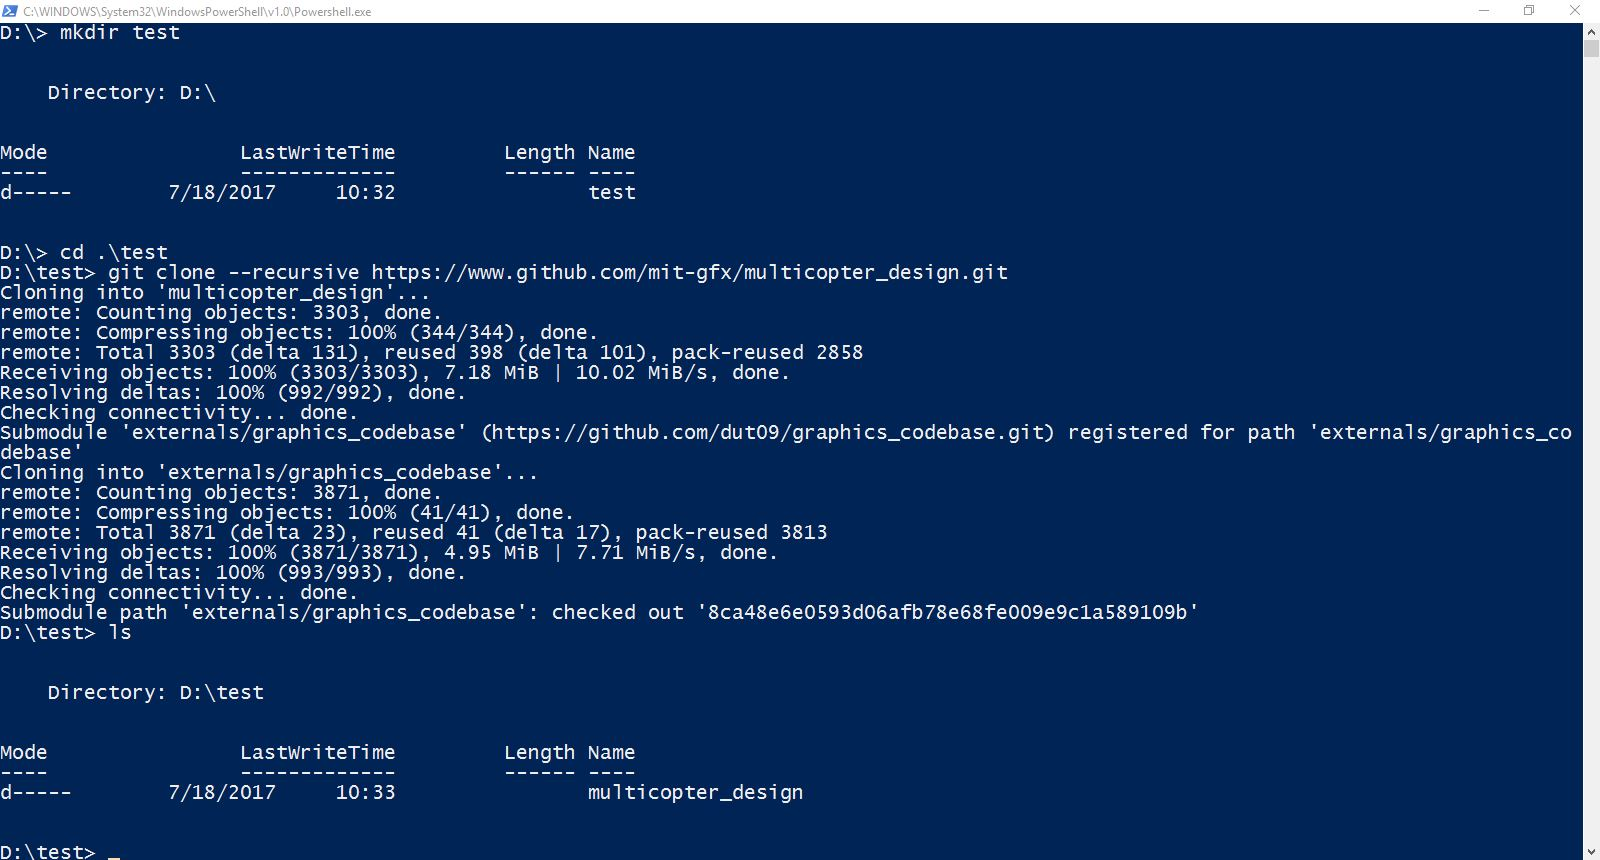
\includegraphics[width=0.75\linewidth]{windows_git_clone}
	\caption{(Windows) Cloning the project into an empty folder named \texttt{test}.}
	\label{fig:windows_git_clone}
\end{figure}

\subsubsection{Download Libraries}
Our program relies on some 3rd party libraries. Please use the provided PowerShell script to download and configure them:
\begin{verbatim}
> cd multicopter_design
> ./windows_setup.ps1
\end{verbatim}

\subsubsection{Generate the Build Solution}
\begin{figure}[!htb]
  \centering
  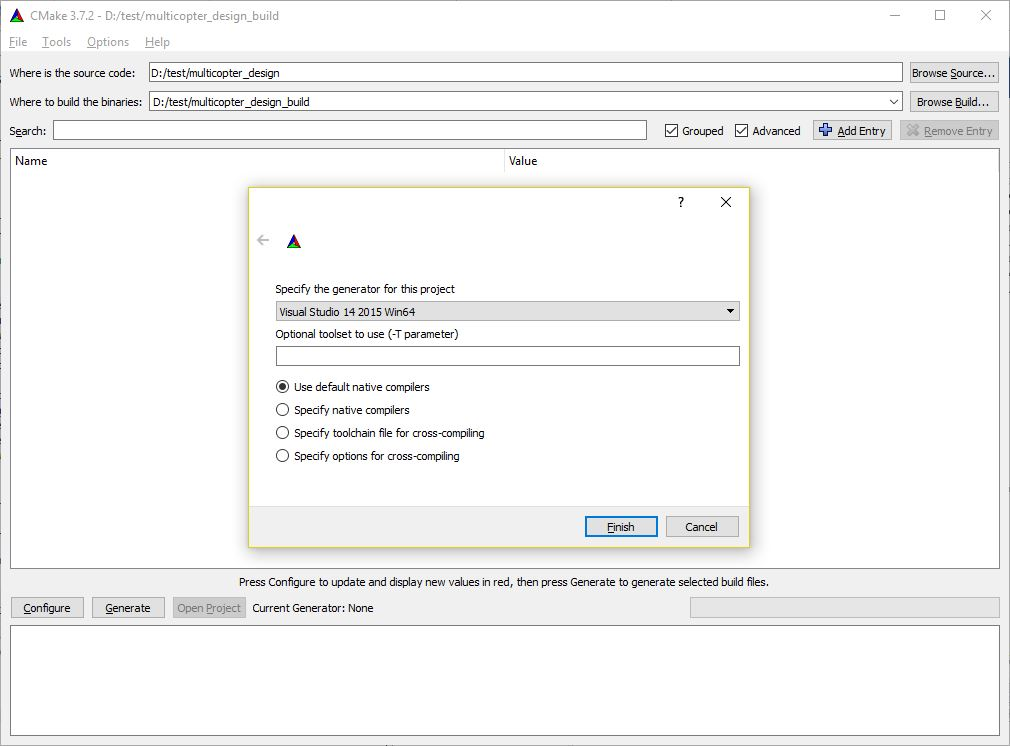
\includegraphics[width=0.75\linewidth]{windows_cmake_code_locations}
  \caption{(Windows) Using CMake to generate the build solution.}
  \label{fig:windows_cmake_code_locations}
\end{figure}
Open CMake GUI. In ``Where is the source code'', type the project location you cloned just now, which is \texttt{D:/test/multicopter\_design} in our case. For ``Where to build the binaries'', use the location you want to put the generated solution file into. Ideally it should be an empty folder out of the source. In our demo we use an empty folder located at \texttt{D:/test/multicopter\_design\_build}. Click ``Configure'', CMake will pop up a window and ask you to choose the generator. Here \texttt{Visual Studio 14 2015 Win64} is select, and you should use the C\texttt{++} IDE you have installed on your computer (Figure~\ref{fig:windows_cmake_code_locations}), click ``Finish'' when you are ready.

During the configuration step, CMake will display a few messages and finally ``Configuring done'' if no error occurs. Click ``Generate'' to create the Visual Studio solution file, which can be found in the location you specified in ``Where to build the binaries''. Click ``Open Project'' and wait for Visual Studio to open your solution.

\subsubsection{Build and Test}
After Visual Studio is open and ready, press \texttt{F7} or click ``Build'' on the menu and choose ``Build Solution''. The default configuration is built in ``Debug'' mode but you can also switch to ``Release'' for faster solution. If no error occurs, multiple executable files will be generated in the folder you used for building binaries. Now set \texttt{copter\_viewer} as the startup project and press \texttt{F5}. A window should pop up and you will see a copter with 5 rotors in the middle (Figure~\ref{fig:windows_default_ui}).
\begin{figure}[!htb]
	\centering
	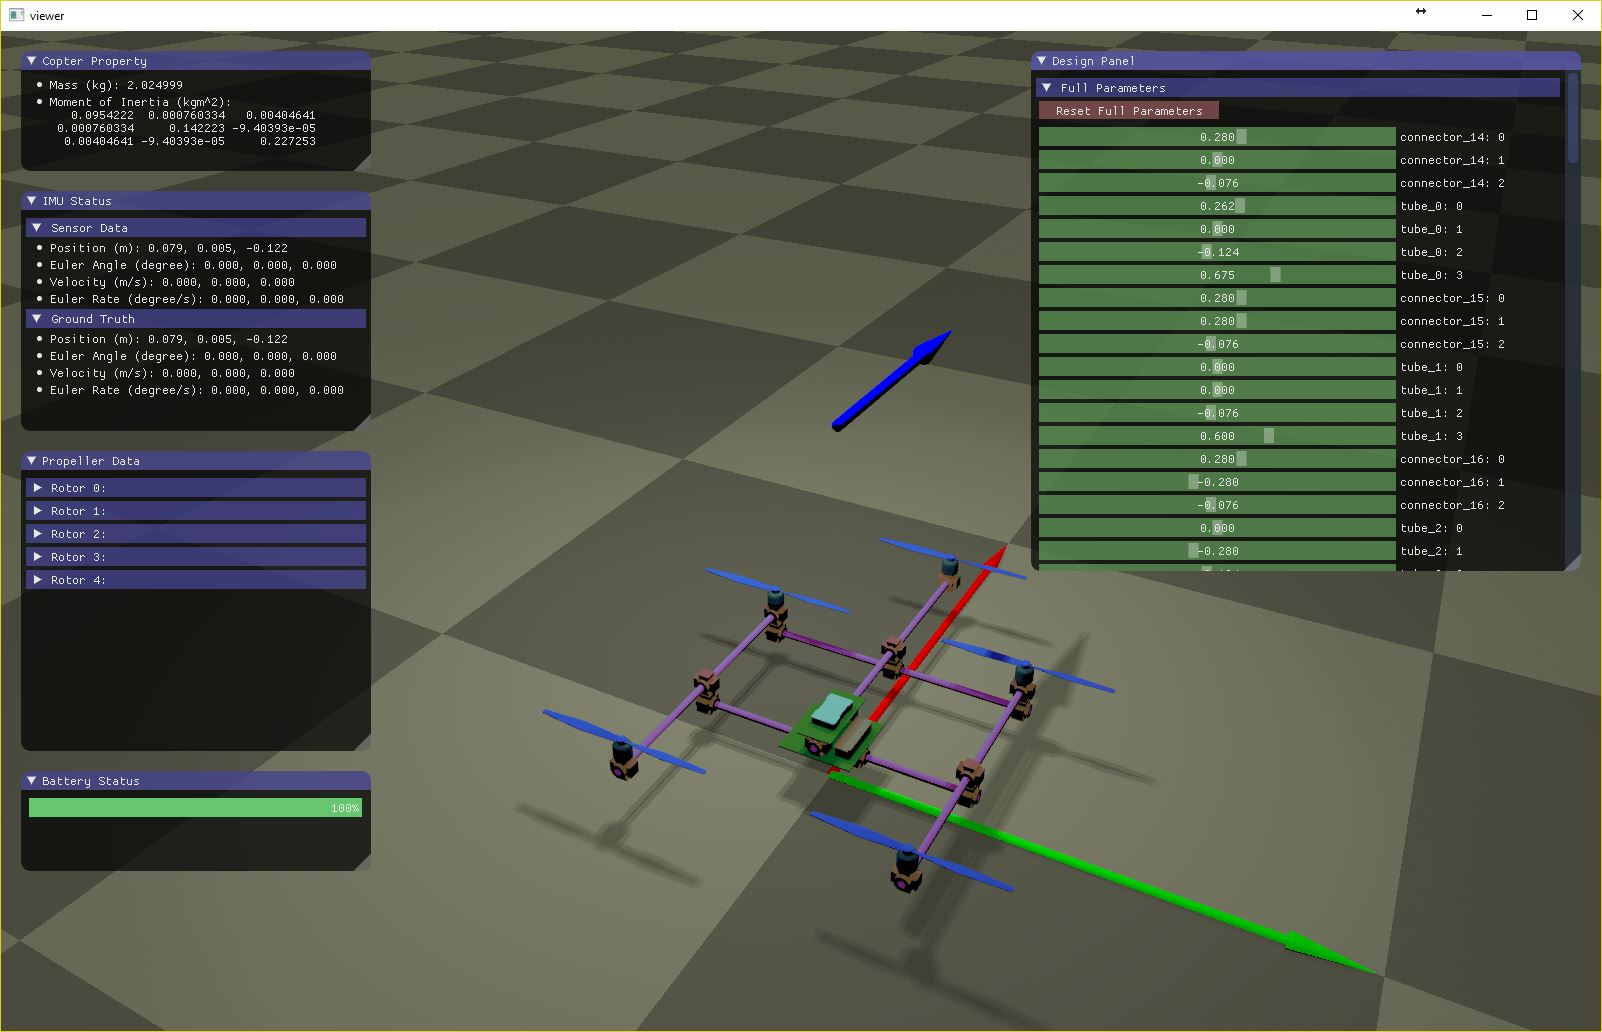
\includegraphics[width=0.75\linewidth]{windows_default_ui}
	\caption{(Windows) A screenshot of the user interface after a successful build.}
	\label{fig:windows_default_ui}
\end{figure}

\subsection{Build on Linux}
This tutorial has been tested on Ubuntu 16.04 LTS 64bit with gcc/g\texttt{++} 4.9.4.

\subsubsection{Install OpenGL libraries} Before you clone our project, make sure all the following libraries have been installed:
\begin{verbatim}
> sudo apt-get update
> sudo apt-get upgrade
> sudo apt-get install libgl1-mesa-dev mesa-common-dev xorg-dev
> sudo apt-get install libglu1-mesa libglu1-mesa-dev
\end{verbatim}
Figure~\ref{fig:ubuntu_opengl_install} is provided for your reference if you encounter any errors and are interested in knowing the exact version of these libraries we are using:
\begin{figure}[!htb]
  \centering
  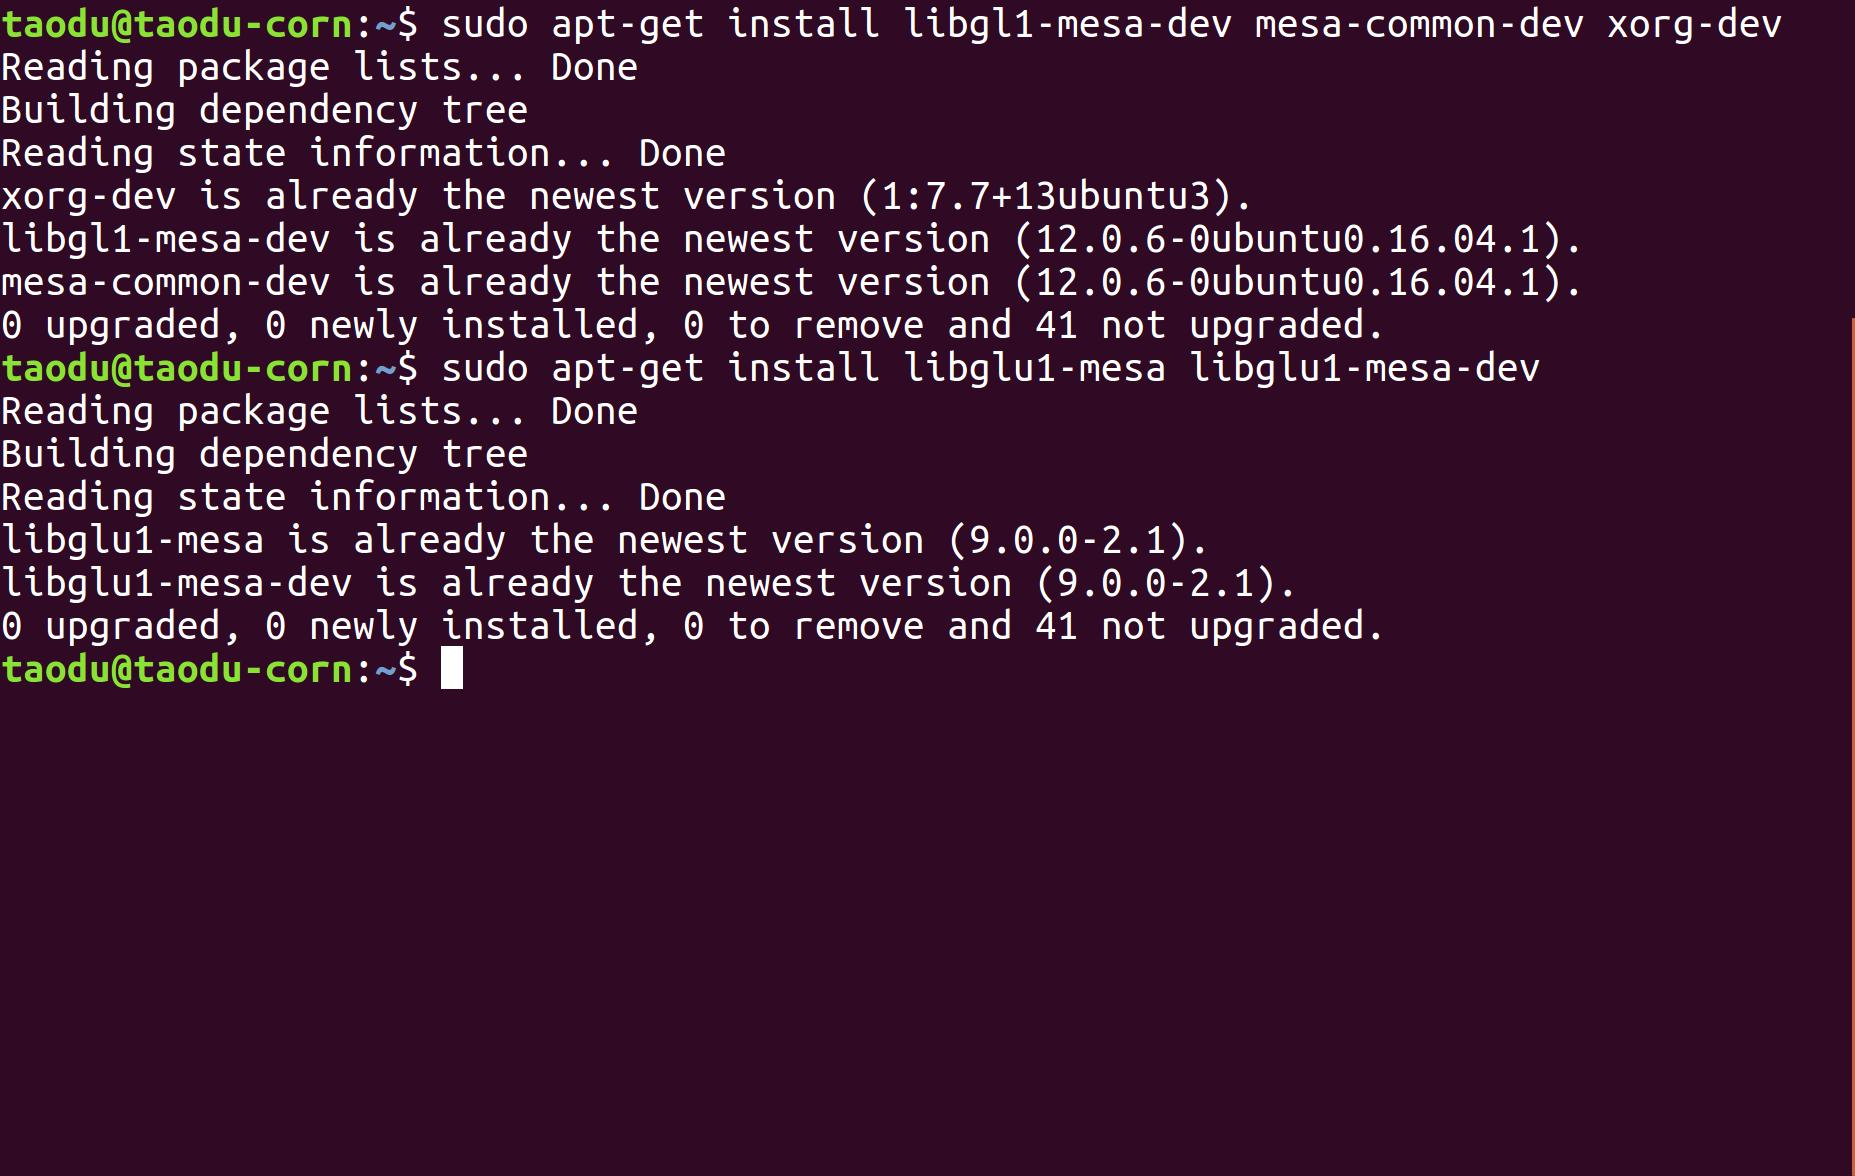
\includegraphics[width=0.75\linewidth]{ubuntu_opengl_install}
  \caption{(Ubuntu) Installing prerequisites.}
  \label{fig:ubuntu_opengl_install}
\end{figure}

\subsubsection{Get the Source Code from GitHub}
Create an empty folder, then use \texttt{git} to clone the project.
\begin{verbatim}
> mkdir test
> cd test
> git clone --recursive https://github.com/mit-gfx/multicopter_design.git
\end{verbatim}

\subsubsection{Download Libraries}
Our program relies on some 3rd party libraries. Please use the provided script to download and configure them:
\begin{verbatim}
> cd multicopter_design
> ./linux_setup.sh
> cd ../
\end{verbatim}

\subsubsection{Generate Makefile}
Next, you will need CMake to generate a Makefile for compiling the code. As before we recommend an out-of-source build. In Figure~\ref{fig:ubuntu_cmake_code_location}, we create an empty folder named \texttt{test/multicopter\_design\_build}, and a Makefile is generated inside.
\begin{verbatim}
> mkdir multicopter_design_build
> cd multicopter_design_build
> cmake ../multicopter_design
\end{verbatim}

\begin{figure}[!htb]
  \centering
  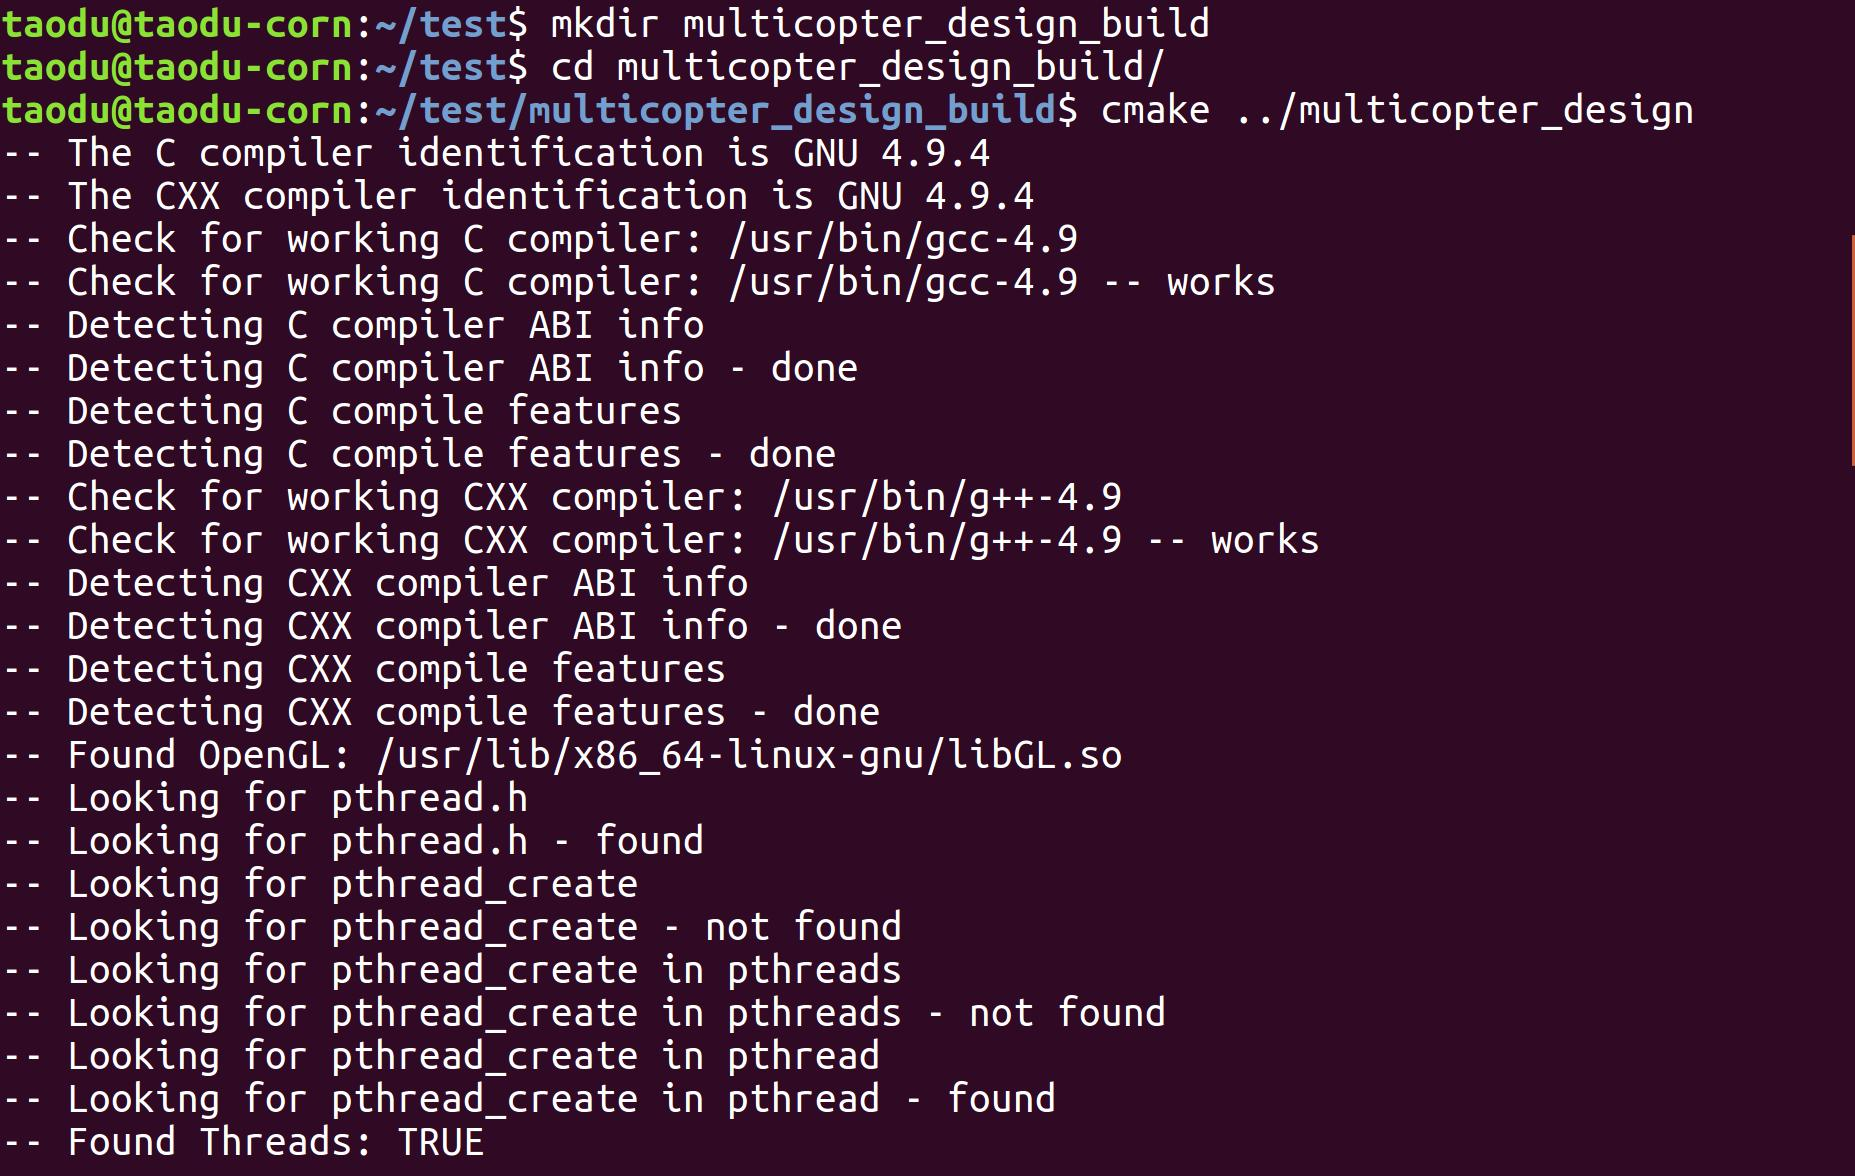
\includegraphics[width=0.75\linewidth]{ubuntu_cmake_code_location}
  \caption{(Ubuntu) Using CMake to generate a Makefile.}
  \label{fig:ubuntu_cmake_code_location}
\end{figure}

\subsubsection{Build and Test}
Once a Makefile is generated, you can call \texttt{make} to build it. If no errors occur, an executable file \texttt{copter\_viewer} will be generated. To test if the build is successful, try running \texttt{copter\_viewer} without any arguments (Figure~\ref{fig:ubuntu_run}), and a window like Figure~\ref{fig:ubuntu_default_ui} should pop up.
\begin{verbatim}
> make
> cd projects/copter_viewer/
> ./copter_viewer
\end{verbatim}

\begin{figure}[!htb]
  \centering
  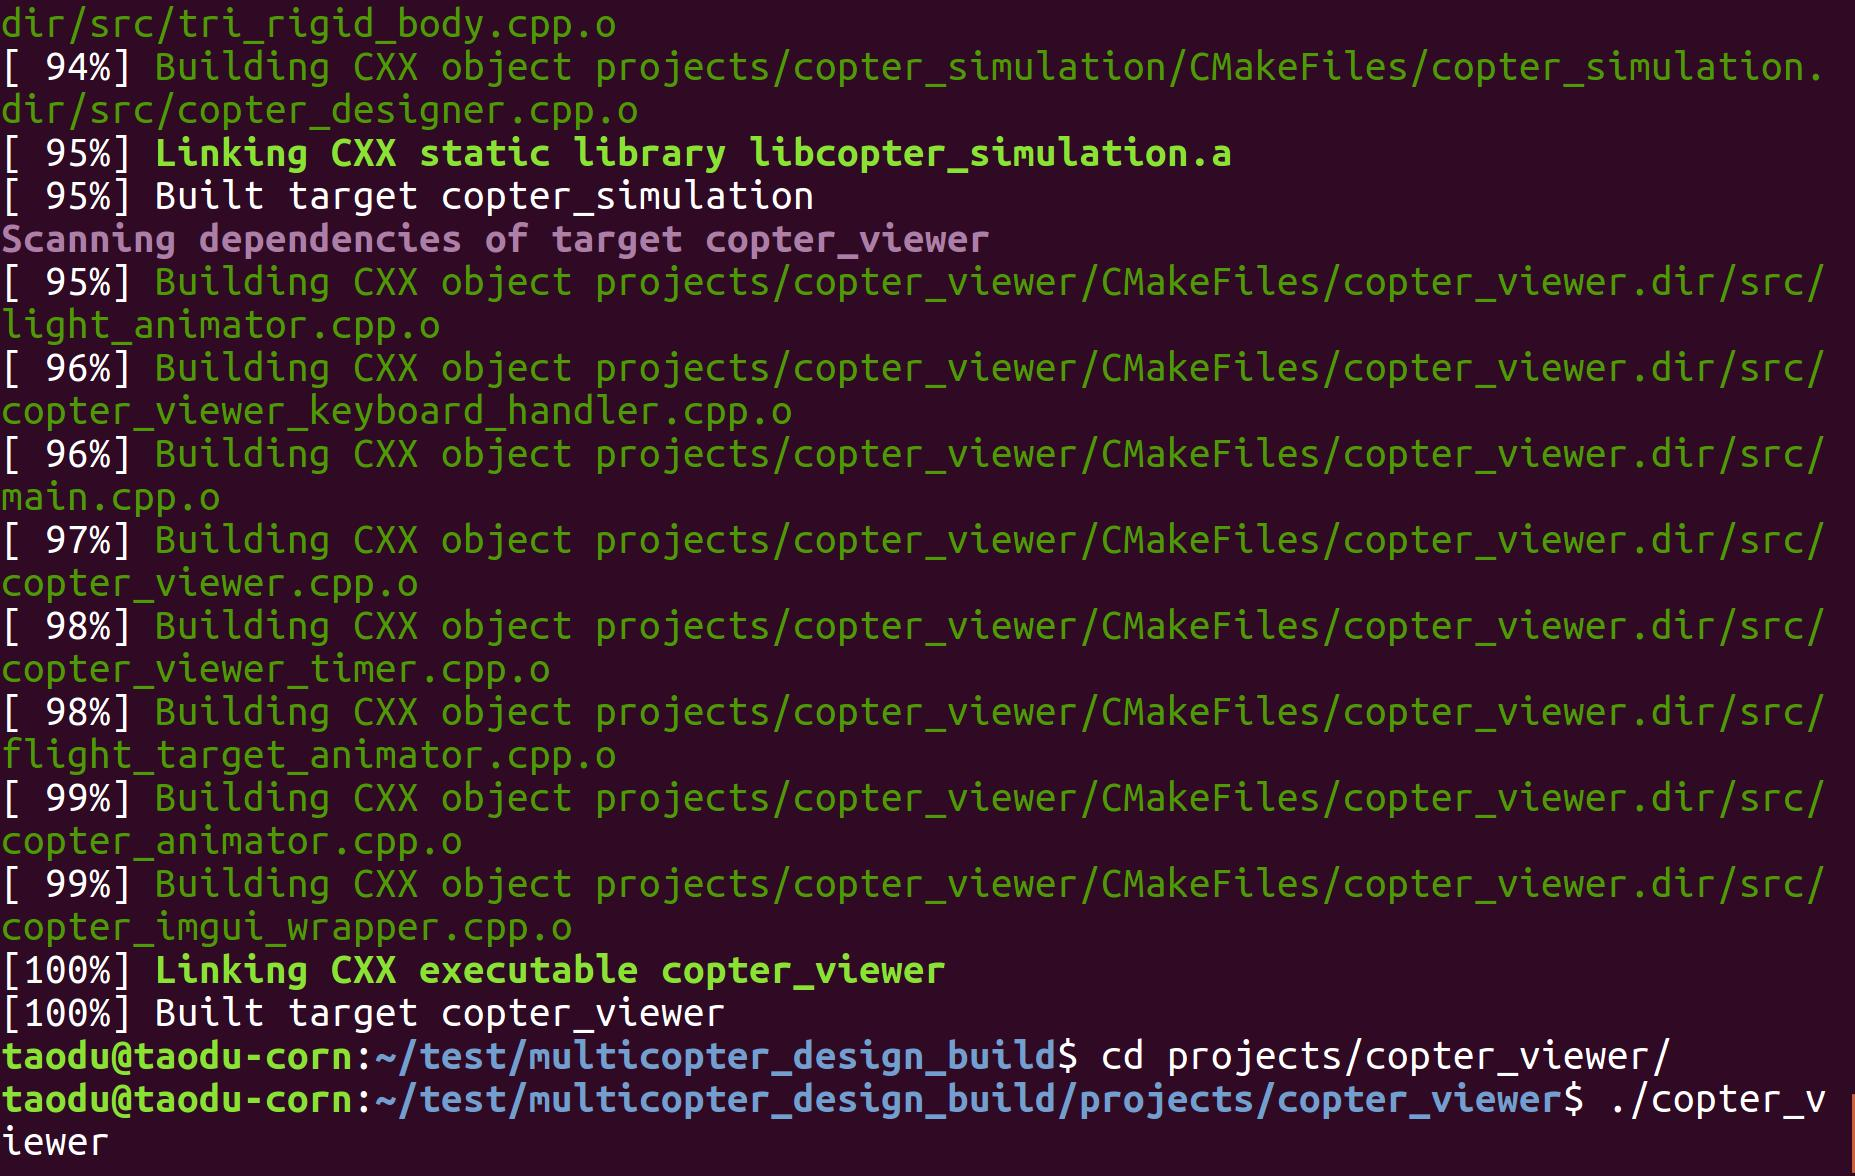
\includegraphics[width=0.75\linewidth]{ubuntu_run}
  \caption{(Ubuntu) Running \texttt{copter\_viewer} without any arguments.}
  \label{fig:ubuntu_run}
\end{figure}
\begin{figure}[!htb]
  \centering
  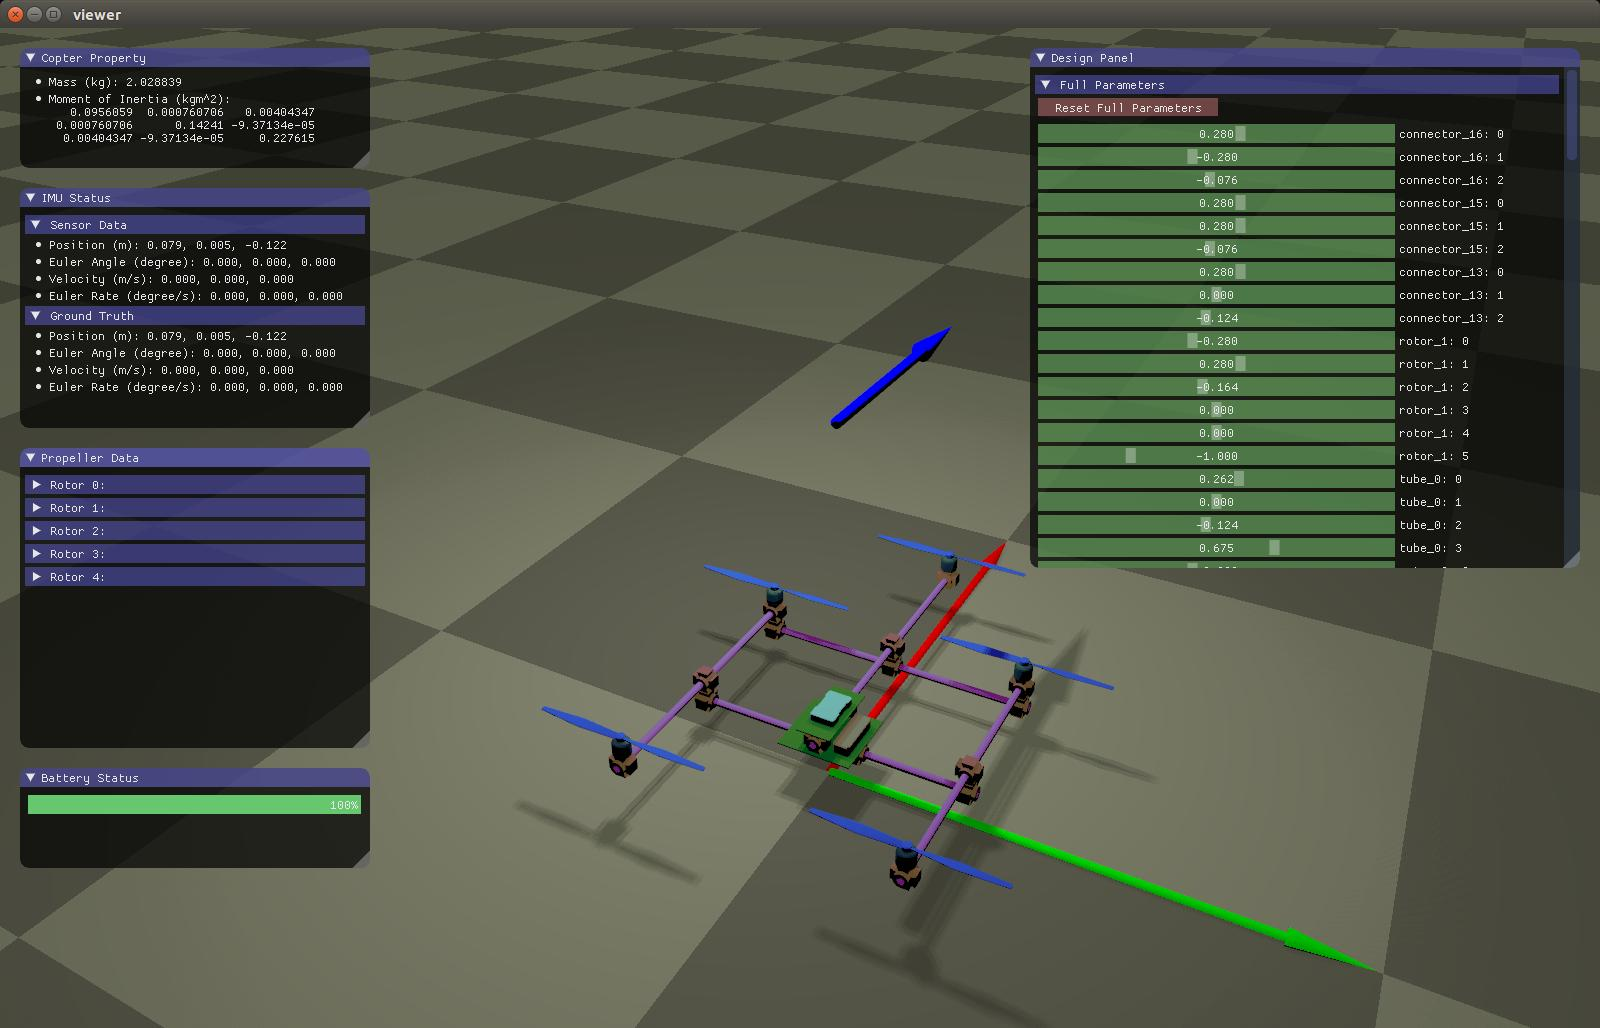
\includegraphics[width=0.75\linewidth]{ubuntu_default_ui}
  \caption{(Ubuntu) A screenshot of the user interface after we build from the source code.}
  \label{fig:ubuntu_default_ui}
\end{figure}

\subsection{Build on macOS}
The following tutorial has been tested on macOS Sierra (10.12.3) with AppleClang 8.1.0 provided in Xcode. The build steps are almost identical to those on Linux, except that no manual OpenGL installation is needed.

\begin{figure}[!htb]
  \centering
  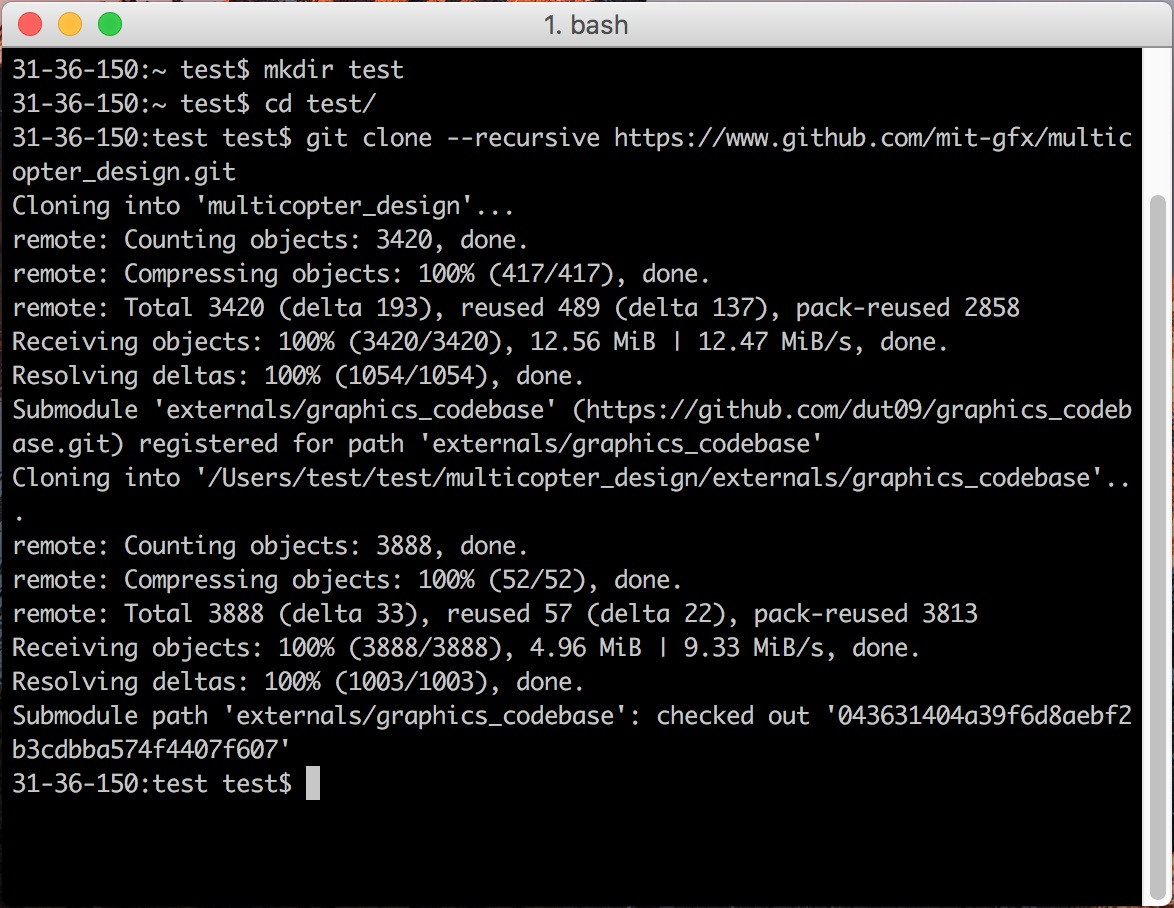
\includegraphics[width=0.75\linewidth]{macos_git_clone}
  \caption{(macOS) Cloning the project into an empty \texttt{test/} folder.}
  \label{fig:macos_git_clone}
\end{figure}
\subsubsection{Get the Source Code from GitHub}
Create an empty folder, then use \texttt{git} to clone the project. In Figure~\ref{fig:macos_git_clone} we cloned it into a newly created empty folder \texttt{test/}:
\begin{verbatim}
> mkdir test
> cd test
> git clone --recursive https://github.com/mit-gfx/multicopter_design.git
\end{verbatim}

\subsubsection{Download Libraries}
Our program relies on some 3rd party libraries. Please use the provided script to download and configure them:
\begin{verbatim}
> cd multicopter_design
> ./macos_setup.sh
> cd ../
\end{verbatim}

\subsubsection{Generate Makefile}
Next, you will need CMake to generate a Makefile for compiling the code. We recommend an out-of-source build. In Figure~\ref{fig:macos_cmake_code_location}, we create an empty folder named \texttt{test/multicopter\_design\_build}, and a Makefile is generated inside.
\begin{verbatim}
> mkdir multicopter_design_build
> cd multicopter_design_build
> cmake ../multicopter_design
\end{verbatim}

\begin{figure}[!htb]
  \centering
  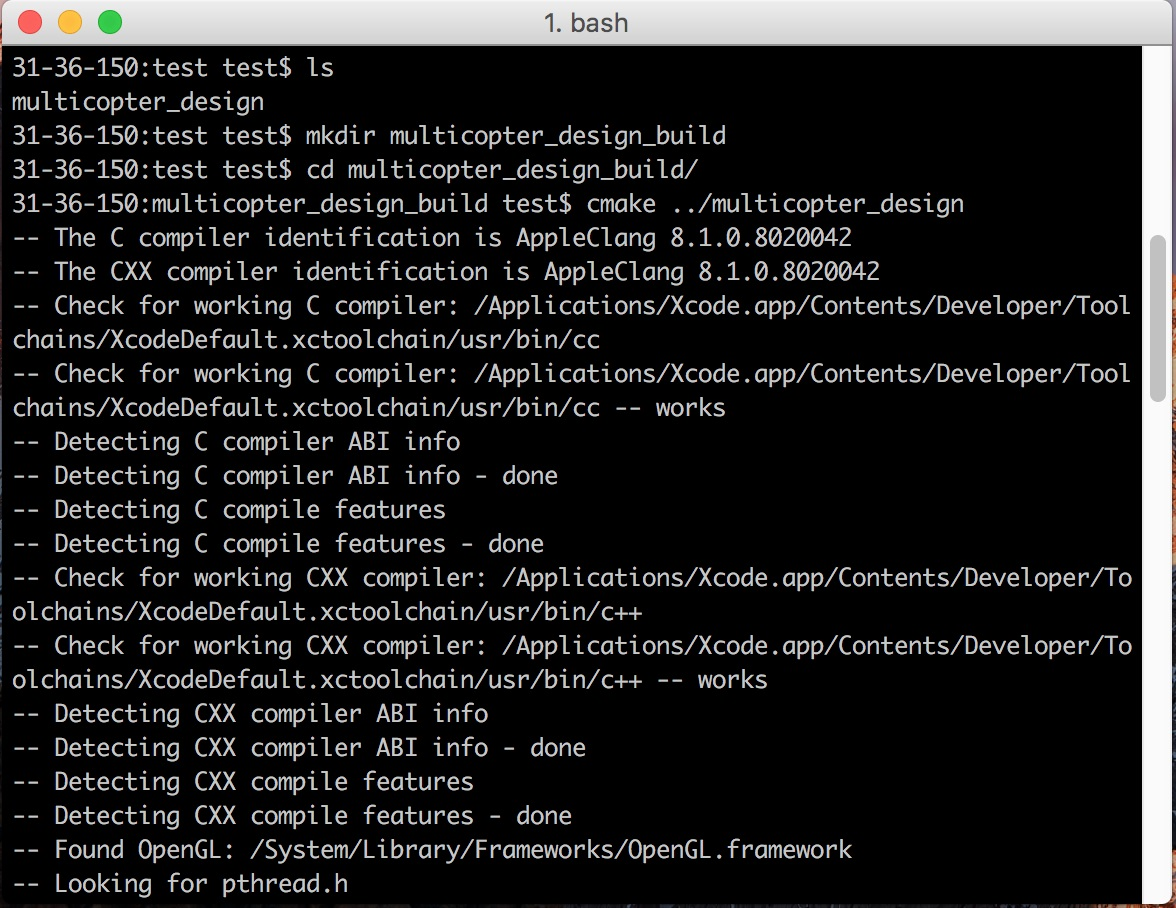
\includegraphics[width=0.75\linewidth]{macos_cmake_code_location}
  \caption{(macOS) Using CMake to generate a Makefile.}
  \label{fig:macos_cmake_code_location}
\end{figure}

\subsubsection{Build and Test}
Once a Makefile is generated, you can call \texttt{make} to build it. If no errors occur, an executable file \texttt{copter\_viewer} will be generated. To test if the build is successful, try running \texttt{copter\_viewer} without any arguments (Figure~\ref{fig:macos_run}), and a window like Figure~\ref{fig:macos_default_ui} should pop up.
\begin{verbatim}
> make
> cd projects/copter_viewer/
> ./copter_viewer
\end{verbatim}
\begin{figure}[!htb]
  \centering
  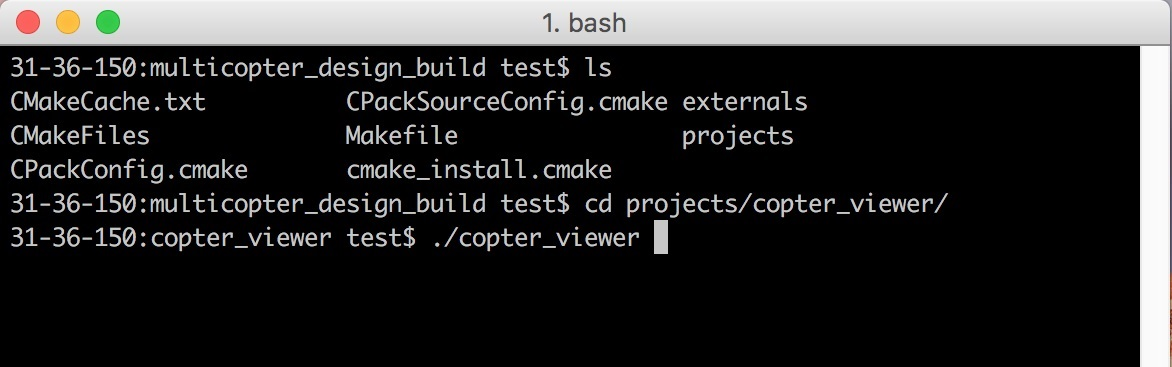
\includegraphics[width=0.75\linewidth]{macos_run}
  \caption{(macOS) Running \texttt{copter\_viewer} without any arguments.}
  \label{fig:macos_run}
\end{figure}

\begin{figure}[!htb]
  \centering
  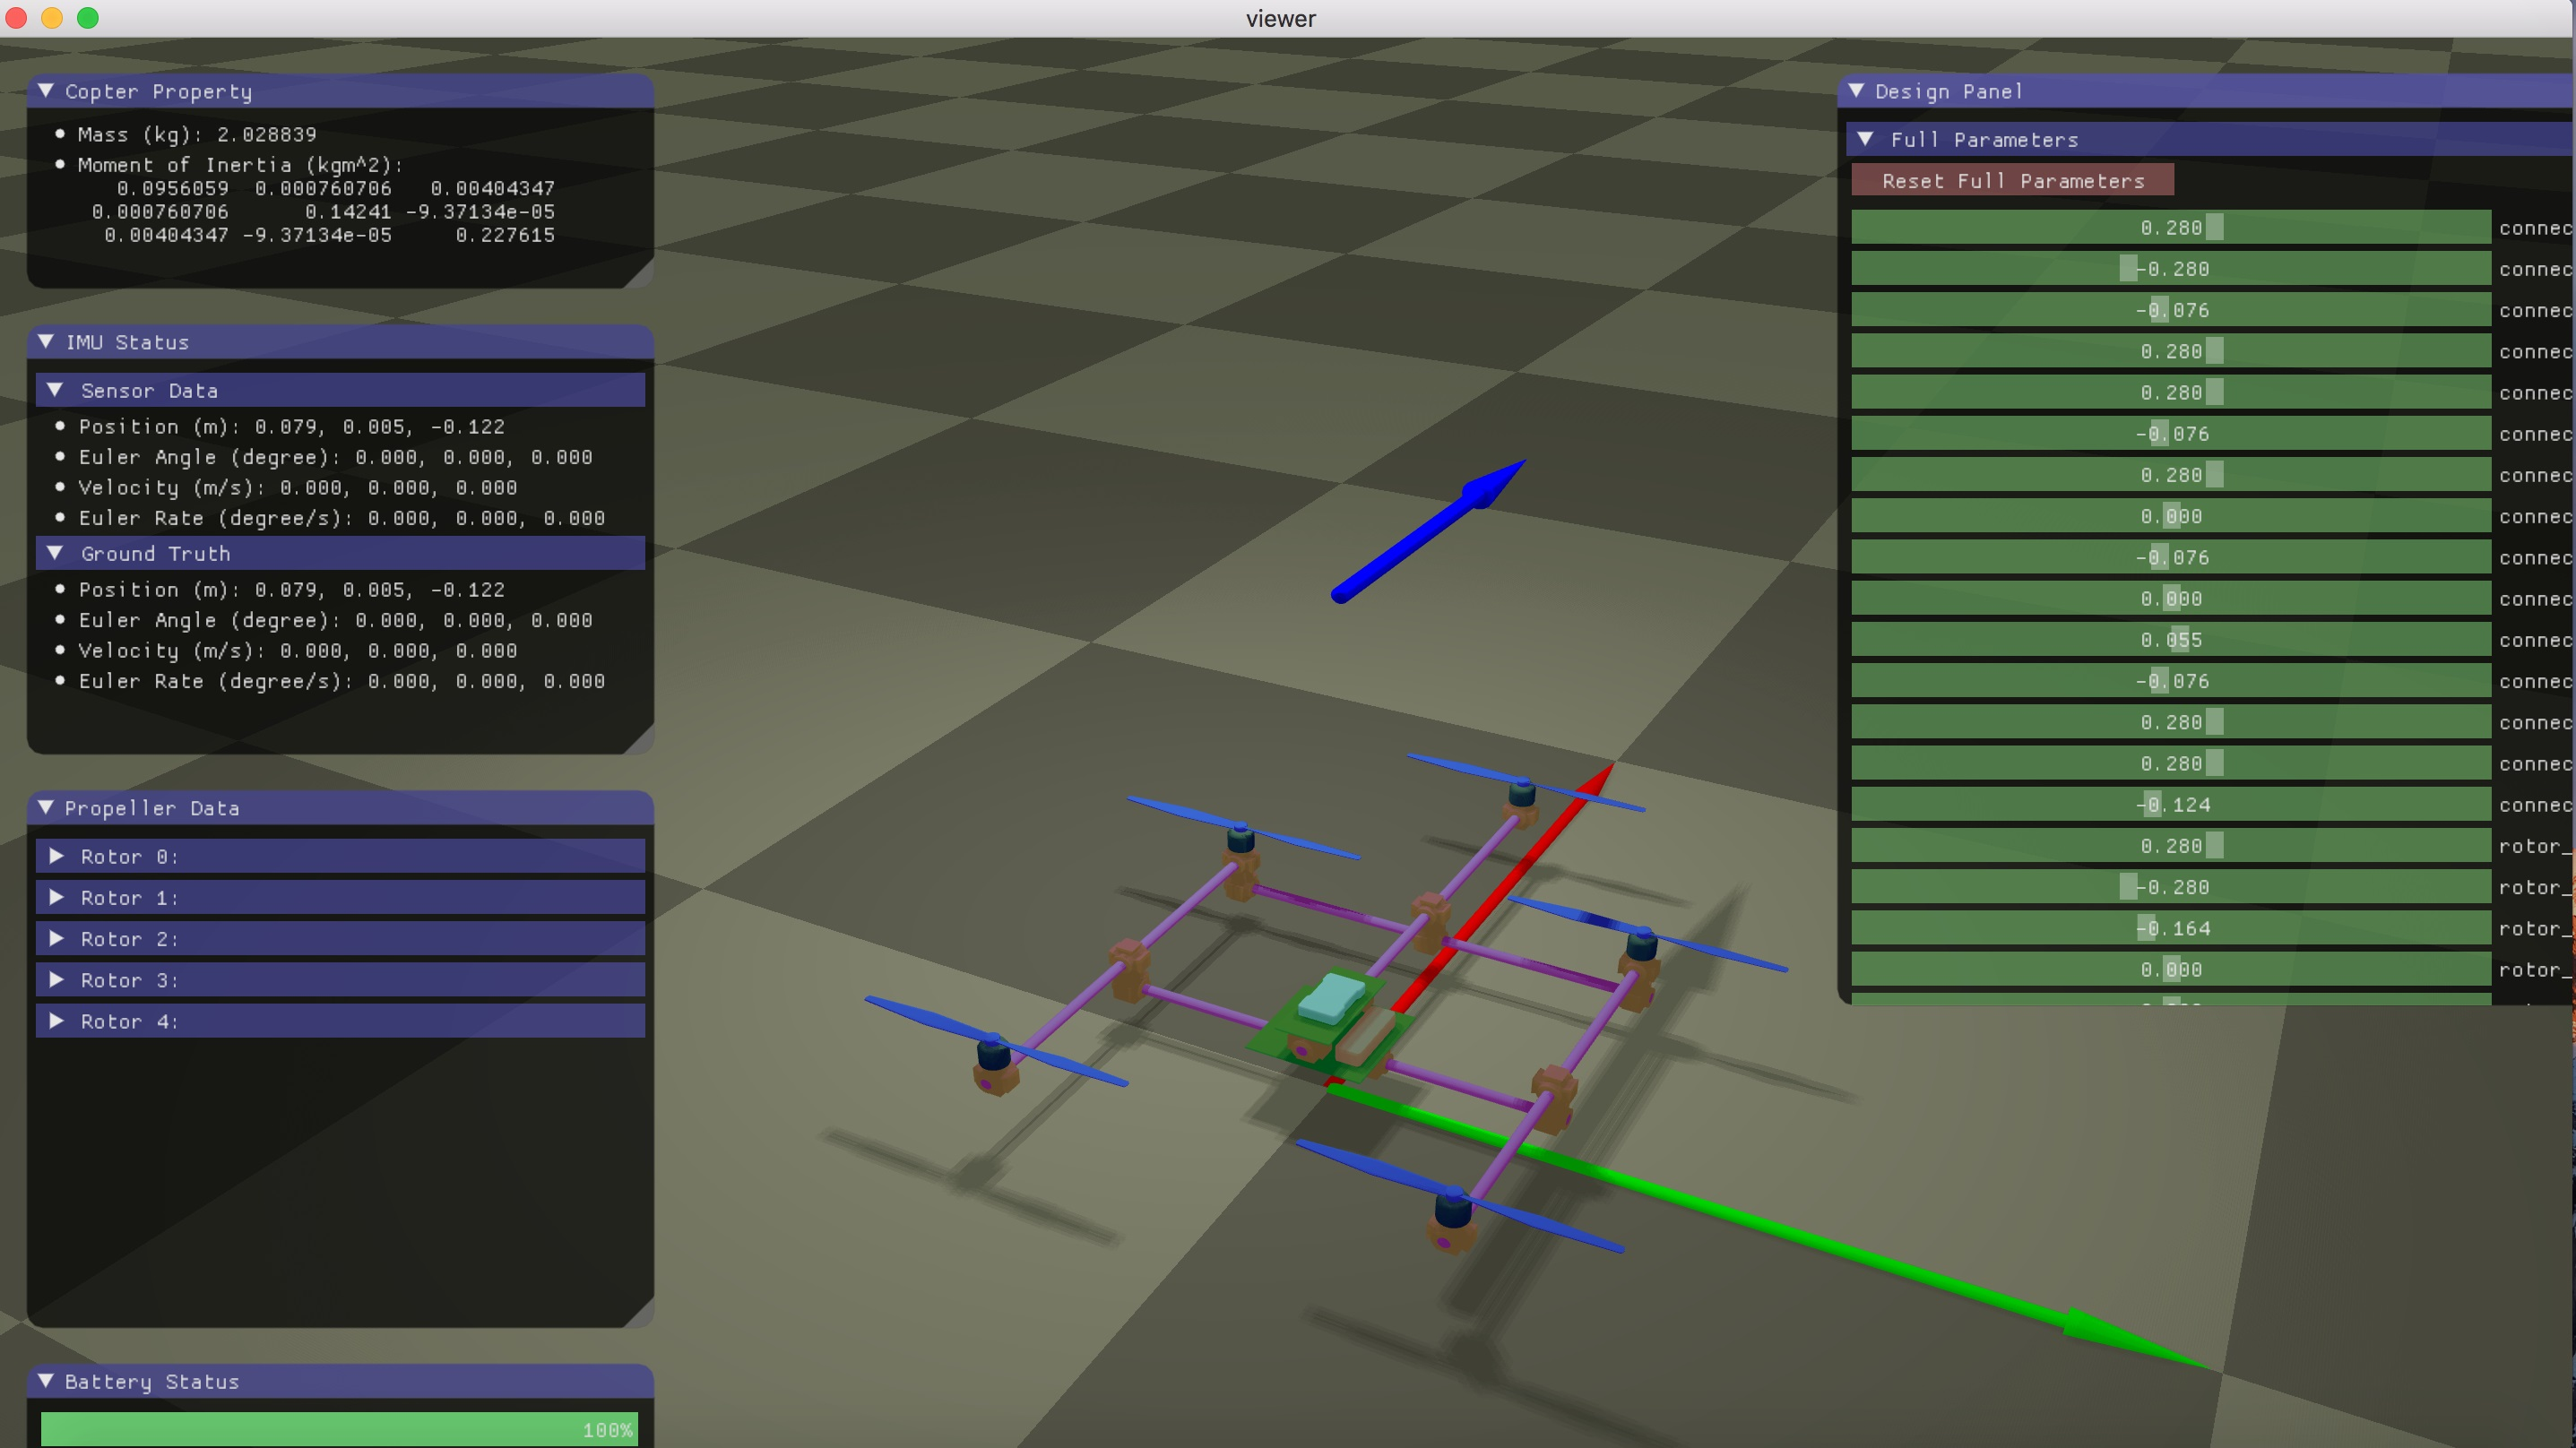
\includegraphics[width=0.75\linewidth]{macos_default_ui}
  \caption{(macOS) A screenshot of the user interface after we build from the source code.}
  \label{fig:macos_default_ui}
\end{figure}